\chapter[Linear Algebra]{Linear algebra} \label{linear_algebra} 

Recall the philosophy of C: the language provides only the most basic of
basics, such as addition and division, and everything else one would
want to do is provided by a function library. Most of statistical analysis is
described as operations on matrices and vectors, so the first key
extension a mathematician needs is a package to do basic vector and
matrix maintenance and linear algebra.

\index{GSL|see{GNU Scientific Library}}
There are many on the market; this chapter uses the \ind{GNU Scientific
Library} (GSL). The GSL is recommended because it is actively supported
and will work on about as many platforms as C itself. The full reference
documentation is readily available online or in book form
\citep{gough:gsl}.

\section{The GSL's matrices and vectors}
As you saw in Chapter \ref{c_crash}, arrays and matrices can be directly implemented in C, but 
the rest of the book will be sticking to the GSL's matrix and vector objects.
If you like using raw arrays better, it's easy to switch back and forth; see
section \ref{asst_conversions}.


\cindex{gsl\_matrix}
\cindex{gsl\_matrix\_set}
\cindex{gsl\_matrix\_set\_row}
\cindex{gsl\_matrix\_set\_col}
\cindex{gsl\_matrix\_alloc}
\cindex{gsl\_matrix\_get}
\cindex{gsl\_vector\_alloc}
\cindex{gsl\_matrix\_free}
\cindex{gsl\_vector\_free}
\index{declaration!of gsl\_matrix@of \ci{gsl\_matrix}}
\index{declaration!of gsl\_vector@of \ci{gsl\_vector}}
\index{for@\ci{for}!example of}
Here is a complete program that will do a few useless things to a few sample
objects:\label{gslexample}
\begin{lstlisting}
#include <gsl/gsl_matrix.h>
#include <stdio.h>

int main(void){
   gsl_matrix   *m = gsl_matrix_alloc(10,10);
   gsl_vector   *v = gsl_vector_calloc(10);
   int  i;

   for (i=0;i< m->size1; i++){
      gsl_matrix_set(m, i, 0, i) ;
   }
   printf("Here is point (3,0): %g\n", gsl_matrix_get(m, 3,0));
   gsl_matrix_set_row(m, 3, v);
   printf("Here is point (3,0) again: %g", gsl_matrix_get(m, 3,0));
   gsl_matrix_free(m);
   gsl_vector_free(v);
   return 0;
}
\end{lstlisting}
\paragraph{A walk through the code}
Here is what just happened: we allocated a 10$\times$10 matrix and a vector of
length 10.  For the sake of variety, we  allocated the two differently.
\ci{gsl\_matrix\_alloc} simply set aside a block of memory for the matrix,
and that block may have garbage in it. Meanwhile, \ci{gsl\_vector\_calloc} set
aside some space for the vector \ci{v}, and set all the values of \ci{v} to
zero.  We were able to do these allocations in the declaration itself.

That done, the \ci{for} loop put some values in the first column of the matrix (leaving garbage in the rest of the matrix). 
The syntax should be familiar to you from section \ref{for_loops}: start at
zero, not one, and increment up to the size of the matrix, which in this case is
\ci{m-$>$size1}. You will recognize this as accessing a structure, which is exactly
what we are doing: the declaration \ci{gsl\_matrix *m} means that
\ci{m} is a pointer to a \ci{gsl\_matrix}, a structure
studied in detail in Section \ref{gslinternals}. For now, only
the two elements \ci{size1} and \ci{size2} are relevant,
indicating the row and column sizes of the matrix. [Row always comes first,
then Column, just like the order in Roman Catholic, Randy Choirboy,
or RC Cola.] Since the vector has only one dimension, the analogous
element of the vector structure is \ci{v-$>$size}.

Next, we copied the vector to the third row of the matrix using \ci{gsl\_\-ma\-trix\_\-set\_\-row(m, 3, v)}. Notice that in so doing, we
overwrote the three at the point (3,0) of the matrix with a zero from
the third element of \ci{v}.

Finally, we freed the memory used for the vectors. This is not 
necessary for a small program,
but it's a good habit to get into for
when you start doing the monolithic analyses, which you may not be
able to run if you don't keep the memory clear of debris.

\paragraph{Naming conventions}  \index{naming functions}
Every function in the GSL library will begin with \ci{gsl\_}, and
the first argument of all of these functions will be the object to be acted upon.
Every function which affects a matrix will begin with \ci{gsl\_matrix\_}
and similarly with vectors and their functions, which all begin with \ci{gsl\_vector\_}. 
Apophenia generally sticks to this as well, and 100\% of its functions
begin with \ci{apop\_} and a great majority of them begin with a data
type such as \ci{apop\_data\_}, \ci{apop\_est\-i\-mate\_}, \&c.

The consistency of the naming means that you have more to type, but
less to memorize. Given the package-object-verb form, you can likely
guess the name of the function you want. Your text editor probably has
some sort of name completion command, which you may want to look up. E.g.,
vim users, try $<$ctrl-n$>$ after typing a few characters. Also, they
make the index very helpful: the index of the GSL's online reference
gives a complete list of functions that operate on vectors alphabetized
under \ci{gsl\_vector\_...}, and the index of this book gives a partial
list of the most useful functions.

\exercise{Don't delay---have a look at the \ci{gsl\_vector\_...}
and \ci{gsl\_matrix\_...} sections of the index to this book or the GSL's online
reference and skim over the sort of operations you can do. The Apophenia
package has a number of higher-level operations that are also worth
getting to know, so have a look at the \ci{apop\_vector\_...}
and \ci{apop\_matrix\_...} sections as well.}

If you find the naming scheme to be too verbose, you can 
write your own wrapper functions that require less typing. For example, you
could write a file \ci{my\_convenience\_fns.c}, which could include:

\cindex{gsl\_matrix\_get}
\cindex{gsl\_matrix\_set}
%\begin{verbatim}
\begin{lstlisting}
double mget(gsl_matrix *m, int row, int col){
   return gsl_matrix_get(m, row, col);
}

double vget(gsl_vector *v, int row){
   return gsl_vector_get(v, row);
}
\end{lstlisting}
%\end{verbatim}

You will also need a header file, \ci{my\_convenience\_fns.h}:
%\begin{verbatim}
\begin{lstlisting}
double mget(gsl_matrix *m, int row, int col);
double vget(gsl_vector *v, int row);
\end{lstlisting}
%\end{verbatim}

After throwing an \ci{\#include "my\_convenience\_fns.h"} at the top of your
program, you will be able to use your abbreviated syntax such as \ci{vget(v,3)}.
It's up to your \ae sthetics as to whether your code will be more or less
legible after you make these changes, but you will need to remember to
bring your convenience functions with you everywhere you go.


\subsection{The easy stuff} The simplest operations on matrices and
vectors are element-by-element, such as adding the elements of one
matrix to those of another. The GSL provides the functions you would
expect to do such things. Each modifies its first argument.
\cindex{gsl\_matrix\_add} \cindex{gsl\_matrix\_sub}
\cindex{gsl\_matrix\_mul\_elements} \cindex{gsl\_matrix\_div\_elements}
\cindex{gsl\_vector\_add} \cindex{gsl\_vector\_sub}
\cindex{gsl\_vector\_mul} \cindex{gsl\_vector\_div}
\cindex{gsl\_matrix\_scale} \cindex{gsl\_matrix\_add\_constant}
\cindex{gsl\_vector\_scale} \cindex{gsl\_vector\_add\_constant}
\lstset{texcl=true} %For this whole section.
\begin{lstlisting}
gsl_matrix_add (a,b);   // $a_{ij} = a_{ij} + b_{ij}, \forall\ i, j$
gsl_matrix_sub (a,b);   // $a_{ij} = a_{ij} - b_{ij}, \forall\ i, j$
gsl_matrix_mul_elements (a,b);  // $a_{ij} = a_{ij} \cdot b_{ij}, \forall\ i, j$
gsl_matrix_div_elements (a,b);// $a_{ij} = a_{ij} / b_{ij}, \forall\ i, j$
gsl_vector_add (a,b);   // $a_{i} = a_{i} + b_{i}, \forall\ i$
gsl_vector_sub (a,b);   // $a_{i} = a_{i} - b_{ij}, \forall\ i$
gsl_vector_mul (a,b);  // $a_{i} = a_{i} \cdot b_{i}, \forall\ i$
gsl_vector_div (a,b);   // $a_{i} = a_{i} / b_{i}, \forall\ i$

gsl_matrix_scale (a,x); // $a_{ij} = a_{ij} \cdot x, \forall\ i, j$, $x\in \Re$
gsl_matrix_add_constant (a,x);  // $a_{ij} = a_{ij} + x, \forall\ i, j$, $x\in \Re$
gsl_vector_scale (a,x); // $a_{i} = a_{i} \cdot x, \forall\ i$, $x\in \Re$
gsl_vector_add_constant (a,x);  // $a_{i} = a_{i} + x, \forall\ i$, $x\in \Re$
\end{lstlisting}

Notice that the functions to multiply and divide two matrices are given
slightly lengthier names to minimize the potential that they will be
confused with the process of multiplying a matrix with another matrix,
${\bf A}{\bf B}$, or its inverse, 
${\bf A}{\bf B}^{-1}$. Those operations require more computational firepower, which
is provided by the BLAS.

\summary{
\item You can express matrices and vectors via \ci{gsl\_matrix} and
\ci{gsl\_vector} structures.
\item Allocate these structures using \ci{gsl\_matrix\_alloc(size1,
size2)} and \ci{gsl\_vector\_alloc(size)}; free them using
\ci{gsl\_matrix\_free(m)} and \ci{gsl\_vector\_free(v)}.
\item Refer to elements using \ci{gsl\_matrix\_set} and
\ci{gsl\_matrix\_get} (and similarly for vectors).
\item Once your data is in these forms, you can operate on the matrix or
vector as a whole using functions like
\ci{gsl\_matrix\_add (a,b)} or \ci{gsl\_vector\_scale (a,x)}.
}

\section{The \ind{BLAS}} 
\index{matrices!dot product|(} \index{dot product|(}
Before there was the GSL, there was the BLAS---the basic linear algebra
system. The GSL has a few functions to interact with the BLAS. In fact,
it has 86. This section covers the three that you will actually 
use.\footnote{The names of the functions here fit in with the system
for the other 83 functions you won't ever use. For example,
\ci{gsl\_blas\_dgemv} is a combination
of D=double precision, GE=general, M=matrix, V=vector.}

Apophenia provides a convenience function, \cind{apop\_dot}, that can
save you from a great deal of the below (see page \pageref{apopdot}).
Therefore, you may prefer to skim this section, and are again
discouraged from memorizing any of it.

\paragraph{Matrix $\cdot$ vector} Here is the header for the function you will use to calculate the dot product of a
matrix and a vector:
\cindex{gsl\_blas\_dgemv|(}
\begin{lstlisting}
int gsl_blas_dgemv (CBLAS_TRANSPOSE_t TransX, float alpha, 
          const gsl_matrix * X, const gsl_vector * v, 
          float beta, gsl_vector * y);
\end{lstlisting}

This will put into the vector $\yv$ either the value 
$\yv \leftarrow \alpha X \vv + \beta \yv$ or $\yv \leftarrow \alpha X' \vv + \beta \yv$, as determined by the
first argument.
\ci{CBLAS\_TRANSPOSE\_t} is a type defined by the GSL that can take
one of two values: \ci{CblasNoTrans} and \ci{CblasTrans}. If
it takes the former value, then $\Xv$ is left alone;
if it takes the latter, it is transposed to $\Xv'$.

To give a concrete example, assume you have already got some vectors and matrices which have the following
declarations:
\begin{lstlisting}
gsl_vector *beta, *gamma;     
gsl_matrix *x, *y;           
\end{lstlisting}

Then, to calculate $\Xv\cdot \betav$, we'd need:

\begin{lstlisting}
gsl_vector *beta_dot_x      = gsl_vector_calloc(x->size1);
gsl_blas_dgemv (CblasNoTrans, 1.0, x, beta, 0.0, beta_dot_x);
\end{lstlisting}

Notice that we used \ci{calloc}, instead of just \ci{alloc}, because
the system will add $\xv\betav$ to \ci{beta\_dot\_x}, not just write it in,
so \ci{beta\_dot\_x} needs to start as all zeros.
\cindex{gsl\_blas\_dgemv|)}

\paragraph{Vector $\cdot$ vector}\label{ddot}
To find the dot product of two vectors, use this function:
\cindex{gsl\_blas\_ddot}
\begin{lstlisting}
int gsl_blas_ddot (const gsl_vector * x, const gsl_vector * y, double * result);
\end{lstlisting}

\exercise{Write a table displaying the sum of squares $1^2 + 2^2 + 3^2 +
\dots + n^2$ for $n= 1$ through $10$.

\begin{itemize}
\item Write a function that takes in $n$ and
    \begin{itemize}
    \item allocates a \ci{gsl\_vector *v} of size $n$,
    \item fills the vector with $1, \dots, n$,
    \item calculates and returns $\vv \cdot \vv$ using \ci{gsl\_blas\_ddot (v, v, v\_dot\_v)},
    \item and finally frees \ci{v}.
    \end{itemize}
\item Write a loop for $n=1$ through $10$, that calls the above function and then prints $n$
and the returned value.
\item Verify your work, by printing $n(n+1)(2n+1)/6$ alongside your calculation of the sum of squares up to $n$.
\end{itemize}
}


\comment{
For example, 

\begin{lstlisting}
double *beta_dot_gamma;
gsl_blas_ddot (beta, gamma, beta_dot_gamma);
\end{lstlisting}
}

\paragraph{Matrix $\cdot$ matrix}
Finally, to take the dot product of two matrices, use:
\cindex{gsl\_blas\_dgemm|(}
\begin{lstlisting}
int gsl_blas_dgemm (CBLAS_TRANSPOSE_t TransX, 
    CBLAS_TRANSPOSE_t TransY, 
    double alpha, const gsl_matrix * X, const gsl_matrix * Y, 
    double beta, gsl_matrix * dot_product);
\end{lstlisting}
which will calculate \ci{dot\_product} $\leftarrow \alpha op(\Xv) op(\Yv) + \beta$ \ci{dot\_product}. $op(\Xv)$ and
$op(\Yv)$ will be either the matrix or its transpose, as above, depending on whether you choose \ci{CblasTrans}
or \ci{CblasNoTrans}. For example, here is $\Xv'\Yv$:

\begin{lstlisting}
gsl_matrix *x_dot_y      = gsl_matrix_calloc(x->size2, y->size2);
gsl_blas_dgemm (CblasTrans,CblasNoTrans, 1, x, y, 0, x_dot_y);
\end{lstlisting}

To give a more extended example, let us say that we have a \ind{transition matrix}, showing whether one can go from a row state to a
column state. Omitting the labels for now, here is a sample:
\label{twostep}\lstinputlisting{sources/data-markov} 
[This is not really a \ind{Markov matrix}, because its
columns are not normalized to sum to one; the reader will see below that it
still is a valid description of a set of transitions.]

\codefig{markov}{A program to read in a transformation matrix and
display the two-step transformation.}
Figure \ref{markov} shows a complete program to read in this matrix and then output this
count of two-step transitions. The steps should be clear: read the data,
allocate a space for the output, calculate the dot product, and print
the result. It introduces a new data type, \cind{apop\_data} to be
discussed fully in Chapter \ref{apop}. For now, just take it to be a
\ci{gsl\_matrix} with labels. On page \pageref{markovtwo}, the
program is simplified using \cind{apop\_data}-specific functions.
%\label{markovone}\lstinputlisting{sources/markov.c}

Here is the output:
\ns{7}\begin{lstlisting}
    2       3       1       2       2       3
    3       4       3       4       4       4
    2       2       3       3       3       2
    4       5       4       5       5       5
    4       5       4       5       5       5
    4       5       4       5       5       5
\end{lstlisting}
This tells us, for example, that there are three ways to transition from state one to
state two in two steps (1 $\Rightarrow$ 1 $\Rightarrow$ 2, 
1 $\Rightarrow$ 2 $\Rightarrow$ 2,  and 1 $\Rightarrow$ 6 $\Rightarrow$
2).

\exercise{\label{quadq}The quadratic form $\Xv'\Yv\Xv$ appears very frequently in
statistical work. Write a function with the header
\ci{gsl\_matrix *quadratic\_form(gsl\_matrix *x, gsl\_matrix *y);} 
that takes two \ci{gsl\_matrix}es and returns the quadratic form as above. Be sure to check that \ci{y} is square and has the same dimension as \ci{x-$>$size1}.}

\cindex{gsl\_blas\_dgemm|)}

\index{matrices!dot product|)}
\index{dot product|)}
\comment{
\paragraph{Scalars} The GSL provides predictable functions for
interacting vectors or matrices with scalars. Here is code to add one to
and then double all the elements of a matrix and a vector:
\begin{lstlisting}
gsl_matrix_add_constant(a_matrix, 1);
gsl_matrix_scale(a_matrix, 2);

gsl_vector_add_constant(a_vector, 1);
gsl_vector_scale(a_vector, 2);
\end{lstlisting}
\cindex{gsl\_matrix\_add\_constant} \cindex{gsl\_matrix\_scale}
\cindex{gsl\_vector\_add\_constant} \cindex{gsl\_vector\_scale}
}

\summary{
\item Matrix $\cdot$ vector: \ci{gsl\_blas\_dgemv}.
\item Matrix $\cdot$ matrix: \ci{gsl\_blas\_dgemm}.
\item Vector $\cdot$ vector: \ci{gsl\_blas\_ddot}.
}

\section{Matrix inversion and equation solving}  \index{matrices!inversion}\index{matrices!determinants}
Matrix inversion is one of the most computationally intensive problems
around. In fact, some will tell you it is the problem for which computers were invented.
Here in the modern day, it is not such a big deal: my old laptop will
invert a $1,000 \times 1,000$ matrix in about ten seconds, and does the
inversion step for the
typical OLS inversion, around a $10 \times 10$ matrix at the
most, in a hundredth of a second.
\comment{
\codefig{invertmatrix}{A function that inverts a matrix using via an LU decomposition.}

The GSL does not include a function to directly invert a general matrix:
instead, the user has to go through a triangular decomposition. Figure
\ref{invertmatrix} shows a function to do all of the steps for us.
Examples for using this function are located throughout the book; for
example, see the calculation of OLS coefficients on page \pageref{ols}.

Figure \ref{invertmatrix} is cut and pasted from the Apophenia source
code; \cind{apop\_det\_and\_inv} does indeed invert and calculate the
determinant of an input matrix. This is what \ttind{apop\_OLS} will use if
you ask for covariances.
}

The GSL does not include a function to directly invert a general matrix:
instead, the user has to go through a triangular decomposition.
Apophenia provides a function to go through the process to find
determinants and inverses, named \cind{apop\_det\_and\_inv}.
Examples for using this function are located throughout the book; for
example, see the calculation of OLS coefficients on page \pageref{ols}.
This is the function \ttind{apop\_OLS} will use if you ask for covariances.

\index{Householder solver}
Because inversion is so computationally intensive, you are better off
not doing so.  For example, we often write the OLS parameters as $\betav
=(\Xv'\Xv)^{-1}(\Xv'\Yv)$, but you could implement this as solving
$(\Xv'\Xv)\betav = \Xv'\Yv$, which involves no inversion. If \ci{xpx} is the
matrix $\Xv'\Xv$ and \ci{xpy} is the vector $\Xv'\Yv$, then 
\cind{gsl\_linalg\_HH\_solve}\ci{(xpx, xpy, out-$>$parameters)} will
return $\betav$. This is how \ci{apop\_OLS} will find $\betav$ if it
is all you ask for.

\summary{
\item You can often avoid inverting matrices, but when you must, you can use
\ci{apop\_det\_and\_inv}.
}

\section{Shunting data} \label{asst_conversions} 
There are many facets to dealing with a computer that one would call
tedious, but for me, the most tedious of all is converting data formats.
You can describe a process easily, say `pull the data and find
$\Xv'\Xv$', but the data is in a text file and your function to take dot
products accepts \ci{gsl\_vectors}, and going from one
to the other will take you much more time than calling the function in
the end.

To that end, this section presents
suggestions for converting among the various data formats used in this
book. It is not an exciting
read, and the only new material is that described under Method V; you may
prefer to take the rest of this section as a reference for use as
necessary. Table \ref{conversiontab} provides the key to the method most
appropriate for each given conversion.

From/to pairs marked with a dot are
left as an exercise for the reader; none are particularly difficult, but
may require going through another format; for example, one can go from a
\ci{double[ ]} to an \ci{apop\_data} set via \ci{double[
]} $\Rightarrow$ \ci{gsl\_matrix} $\Rightarrow$ \ci{apop\_data}.
One can go from any format to any other in two steps, as proven above
using the transition matrix and dot product on page \pageref{twostep}. 

\def\rcap#1{\rotatebox{45}{#1}\hskip -15pt }
\def\rcapc#1{\rotatebox{45}{\ci{#1}}\hskip -15pt }
\def\cd{$\cdot$}
\begin{figure} \begin{center}
\begin{tabular}{ll}
\rotatebox[x=15mm]{90}{From}&
\begin{tabular}{lp{0.4cm}p{0.4cm}p{0.4cm}p{0.4cm}p{0.4cm}p{0.4cm}}
   &   &&&To\\
    & \rcap{Text file} & \rcap{Db table} & \rcapc{double[]} 
        & \rcapc{gsl\_vector} & \rcapc{gsl\_matrix}& \rcapc{apop\_data}\\
Text file               & C & F & \cd & \cd & \cd &  F                   \\
Db table                & \cd & Q & \cd & Q & Q & Q                  \\
\ci{double[ ]}      & \cd & \cd & C & F & F & \cd                  \\
\ci{gsl\_vector}   & P  & P & F & C & F & F                    \\
\ci{gsl\_matrix}   &  P & P & F & V &C &  F               \\
\ci{apop\_data}    & P & P & F & S & S &C
\end{tabular}
\end{tabular}
\caption{Methods of conversion} \label{conversiontab}
\end{center}\end{figure} 


\paragraph{Method C: Copying} There are two styles of copying.
One is the family of functions with \cind{memcpy} in the name, that are
of the form \ci{memcpy(dest, src)}.\footnote{Notice that for virtually
all functions throughout the text, the order of the arguments is 
inputs first and then outputs. For basically historical reasons, the
\ci{memcpy} functions are the reverse.} They assume that \ci{dest}
is already allocated.  
Apophenia provides functions to allocate and copy in one step, with
names of the form \ci{apop\_...\_copy}.

\cindex{gsl\_vector\_memcpy} \cindex{gsl\_matrix\_memcpy}
\cindex{apop\_data\_memcpy} \cindex{apop\_data\_memcpy} \cindex{system}
\ns{22}\begin{lstlisting}
//Text file $\Rightarrow$ Text file
//Just use the system's file copy command.
    system("cp %s %s", from_file_name, to_file_name);
//\ci{gsl\_vector} $\Rightarrow$ \ci{gsl\_vector}
    gsl_vector *copy   = gsl_vector_alloc(original->size);
    gsl_vector_memcpy(copy, original);
    gsl_vector *copy2 = apop_vector_copy(original);
//\ci{double[ ]} $\Rightarrow$ \ci{double[ ]}
//You need to know the size of the original.
    double *copy1 = malloc(sizeof(double) * original_size);
    memcpy(copy1, original, sizeof(double) * original_size);
    double copy2[original_size];
    memcpy(&copy2, original, sizeof(double) * original_size);
//\ci{gsl\_matrix} $\Rightarrow$ \ci{gsl\_matrix}
    gsl_matrix *copy   = gsl_matrix_alloc(original->size1, original->size2);
    gsl_matrix_memcpy(copy, original);
    gsl_matrix *copy2 = apop_matrix_copy(original);
//\ci{apop\_data} $\Rightarrow$ \ci{apop\_data}
    apop_data *copy1 = apop_data_alloc(original->matrix->size1, original->matrix->size2);
    apop_data_memcpy(copy1, original);
    apop_data *copy2 = apop_data_copy(original);
\end{lstlisting}

\paragraph{Method F: Function call}
\cindex{apop\_vector\_to\_matrix}\cindex{apop\_vector\_to\_data}\cindex{apop\_matrix\_to\_data}
\cindex{apop\_text\_to\_data} \cindex{apop\_text\_to\_db}
\cindex{apop\_array\_to\_matrix} \cindex{apop\_array\_to\_vector}
\cindex{apop\_line\_to\_matrix} \cindex{apop\_line\_to\_data}
\index{arrays}

These are functions designed to convert one format to another.

There are two ways to express an array of \ci{double}s. One is to
declare a pointer to pointers to \ci{double}s, and the other is to
declare double-subscripts:
\begin{lstlisting}
double **method_one = malloc(sizeof(double*)*size_1);
double method_two[size_one][size_two] = {{2,3,4},{5,6,7}};
\end{lstlisting}
The second method seems convenient, because it lets you allocate the
matrix at once. But due to minuti\ae{} that will not be discussed here
(see \citet[p 113]{kandr:c}), method two is too much of a hassle to
be worth anything. 

Instead, declare your data as a single line, listing the entire first
row, then the second, et cetera, with no intervening brackets. Then, use
the \ci{apop\_line...} functions to convert to a matrix. Below, the
first set of examples convert from an array declared as in method one
above, and the second set shows an array declared as a single line and
then converted to a $2 \times 3$ matrix.
\begin{lstlisting}
//text $\Rightarrow$ db table
//The first number states whether the file has row names; the second
//whether it has column names. Finally, if no colnames are present,
//you can provide them in the last argument as a \ci{char **}
    apop_text_to_db("original.txt", "tablename", 0 , 1, NULL);
//text $\Rightarrow$ \ci{apop\_data}
    apop_data *copy = apop_text_to_data("original.txt", 0 , 1);
//\ci{double[ ]} $\Rightarrow$ \ci{gsl\_vector}
    gsl_vector  *copy = apop_array_to_vector(original, original_size);
//\ci{*double[ ]} $\Rightarrow$ \ci{gsl\_matrix}
    gsl_matrix *copy = apop_array_to_matrix(original, original_size1, original_size2);

//\ci{double[ ]} $\Rightarrow$ \ci{gsl\_matrix}
    double original[] = {2,3,4,5,6,7};
    int original_size1 = 2, original_size2 = 3;
    gsl_matrix *copy = apop_line_to_matrix(original, original_size1, original_size2);
//\ci{double[ ]} $\Rightarrow$ \ci{apop\_data}
    apop_data *copy = apop_line_to_data(original, original_size1, original_size2);

//\ci{gsl\_vector} $\Rightarrow$ \ci{double[ ]}
    double *copy;
    int copy_size   = original_vec->size;
    apop_vector_to_array(original_vec, &copy);
//\ci{gsl\_vector} $\Rightarrow$ \ci{gsl\_matrix}
    gsl_matrix   *copy = apop_vector_to_matrix(original_vec);
//\ci{gsl\_vector} $\Rightarrow$ \ci{apop\_data}
    apop_data   *copy = apop_vector_to_data(original_vec);
//\ci{gsl\_matrix} $\Rightarrow$ \ci{apop\_data}
    apop_data   *copy = apop_matrix_to_data(original_matrix);
\end{lstlisting}

\paragraph{Method P: Printing}
\cindex{apop\_vector\_print} \cindex{apop\_matrix\_print} \cindex{apop\_data\_print}
Apophenia's printing functions will print to screen, text file, or
database, depending on the value of \cind{apop\_opts.output\_type}.
\begin{lstlisting}
//\ci{gsl\_vector} $\Rightarrow$ text file
//\ci{gsl\_matrix} $\Rightarrow$ text file
//\ci{apop\_data} $\Rightarrow$ text file
    apop_opts.output_type = 't'
    apop_vector_print(original_vector, "text_file_copy");
    apop_matrix_print(original_matrix, "text_file_copy");
    apop_data_print(original_data, "text_file_copy");
//\ci{gsl\_vector} $\Rightarrow$ db table
//\ci{gsl\_matrix} $\Rightarrow$ db table
//\ci{apop\_data} $\Rightarrow$ db table
    apop_opts.output_type = 'd'
    apop_vector_print(original_vector, "db_copy");
    apop_matrix_print(original_matrix, "db_copy");
    apop_data_print(original_data, "db_copy");
\end{lstlisting}


\paragraph{Method Q: Querying}
\cindex{apop\_query} \cindex{apop\_query\_to\_vector}
\cindex{apop\_query\_to\_matrix} \cindex{apop\_query\_to\_data}
The only way to get data out of a database is to query it out. Apophenia
provides a function that will produce the appropriate output.

\begin{lstlisting}
//db table $\Rightarrow$ db table
    apop_query("create table copy as \
    select * from original");
//db table $\Rightarrow$ \ci{double}
    double d = apop_query_to_float("select value from original");
//db table $\Rightarrow$ \ci{gsl\_vector}
    gsl_vector *v = apop_query_to_vector("select * from original");
//db table $\Rightarrow$ \ci{gsl\_matrix}
    gsl_matrix *m = apop_query_to_matrix("select * from original");
//db table $\Rightarrow$ \ci{apop\_data}
    apop_data *d = apop_query_to_data("select * from original");
\end{lstlisting}


\paragraph{Method S: Subelements} Sometimes, even a function is just
overkill; you can just pull a subelement from the main data item.

Notice, by the way, that the \ci{data} subelement of a
\ci{gsl\_vector} can not necessarily be copied to a
\ci{double[ ]}---the \airq{stride} may be wrong; see Section
\ref{gslinternals}
for details. Instead, use the copying functions from Method F above.

\begin{lstlisting}
//\ci{apop\_data} $\Rightarrow$ \ci{gsl\_matrix}:
    my_data_set -> matrix
\end{lstlisting}
\lstset{texcl=false}

%\eject

\comment{
\marginaliafixed{18}{Allocating and using at once}{    \index{declaration}
One slight convenience that helps with the annoyance of shunting data from
one type to another is that you can declare a variable and assign it at the
same time. Let us say that you have already filled a \ci{gsl\_matrix
*m} with data and want it to be an \ci{apop\_data} structure. Then
you can declare and allocate your new structure with one line:\\
%\begin{lstlisting}
\ci{apop\_data   *mdata  = apop\_matrix\_to\_data(m);}\\
%\end{lstlisting}
On the left-hand side, we are allocating an \ci{apop\_data *} pointer, and
on the left-hand side, \cind{apop\_data\_from\_matrix} returns an 
\ci{apop\_data *} pointer. As in the example on page \pageref{gslexample}, the same can be
done with any function with \ci{alloc} in the name, because they will also
return a pointer to the appropriate type.
}
}

\paragraph{Method V: Views}\index{views}\index{matrices!views}
The GSL includes a convenient structure, the \vocab{view}, for pulling a vector from a
matrix. Here is how to get the fifth row of \ci{a\_matrix} into a vector view:

\begin{lstlisting}
gsl_vector v;
v = gsl_matrix_col(a_matrix, 4).vector;
apop_vector_show(&v);
\end{lstlisting}
[Notice that this function is named \ci{col}, not \ci{column}.]
For the fifth row, use \ci{gsl\_matrix\_row(a\_\-ma\-trix, 4)}. 
\cindex{gsl\_matrix\_row} 

\begin{figure}[htb]
\begin{center}
\scalebox{0.7}{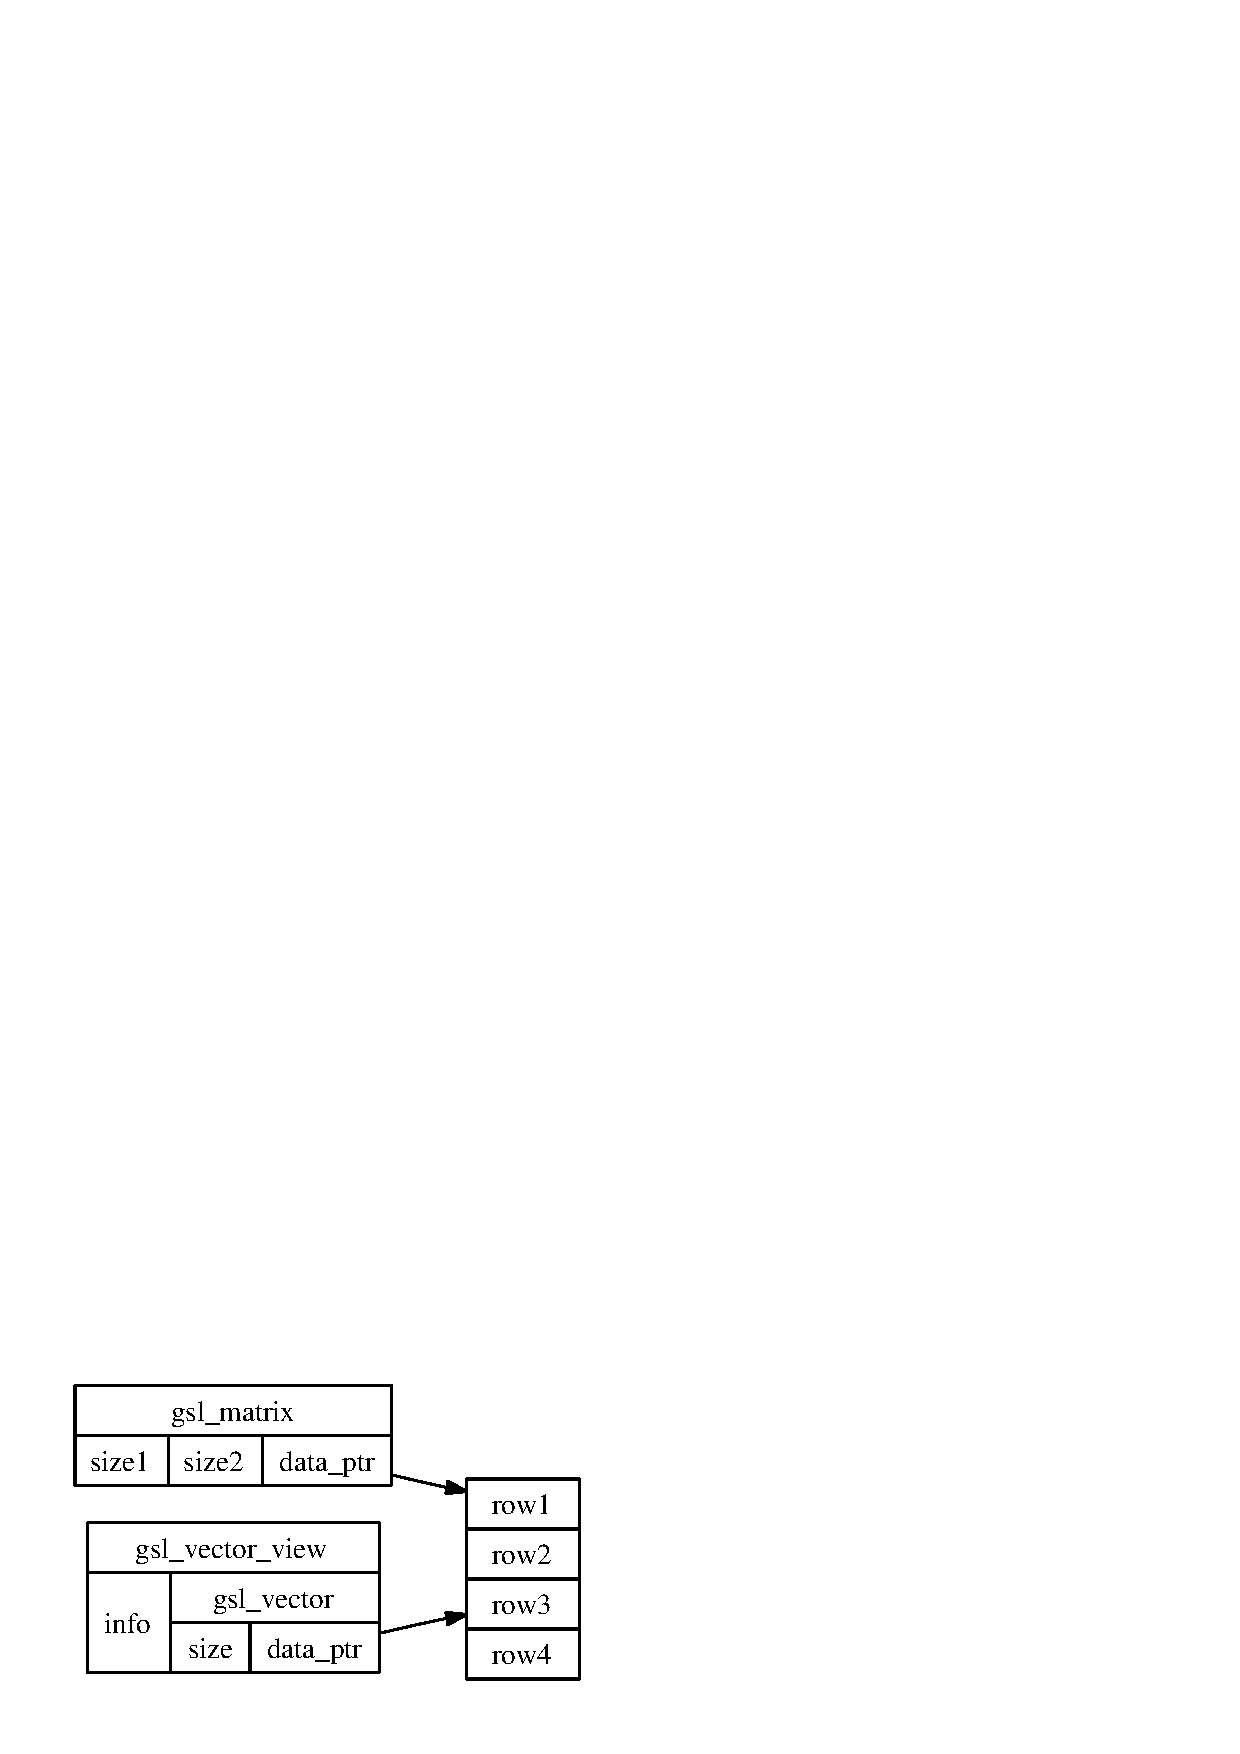
\includegraphics{figs/views}}
\end{center}
\caption{Inside a \ci{gsl\_vector\_view} structure, there is a plain
\ci{gsl\_vector}, which points to a subset of the original data.}
\label{viewfig}
\end{figure}
The vector view is a nice test of your comprehension of the details of
pointers and memory allocation from Section \ref{pointers}.
\ci{gsl\_ma\-trix\_col} returns a
\cind{gsl\_vector\_view}---not a pointer, but the actual
structure.  Inside the \ci{gsl\_vec\-tor\_view}, you will find 
an element named \ci{vector}, which is again not a pointer but an
automatically allocated structure [see Figure \ref{viewfig}]. Inside that \ci{.vector}
element, one would find a pointer to the original data. 

When the function ends, all of the automatically-allocated data is
thrown out, including \ci{gsl\_\-vec\-tor\_\-view} and its
\ci{vector} element, but the data itself is untouched.

Notice further that every function that handles a
\ci{gsl\_\-vec\-tor} actually takes a {\em pointer} to a 
\ci{gsl\_\-vec\-tor}. Thus, the fact that you have an actual 
\ci{gsl\_\-vec\-tor} on your hands means that you will have to pass
its address to the various functions, as in the call to
\ci{apop\_\-vec\-tor\_\-show} above.
\cindex{apop\_vector\_show}

Apopehnia provides a few macros that are significantly less verbose than
the above use of \ci{gsl\_matrix\_row}, but may or may not be more
readable. The macro
\cindex{APOP\_MATRIX\_ROW}
\cindex{APOP\_MATRIX\_COL}
\begin{lstlisting}
APOP_MATRIX_ROW(m, row, v);
\end{lstlisting}
expands to
\begin{lstlisting}
gsl_vector apop_vv_v = gsl_matrix_row(m, row).vector;
gsl_vector *v        = &apov_vv_v
\end{lstlisting}
meaning that the macro declares a typical pointer to a \ci{gsl\_vector},
which can be handled as normal. You will never deal with the
\ci{apop\_vv\_v} variable, and so can ignore it as the internal
machinery that it is.

The main drawback to the \ci{APOP\_MATRIX\_ROW} and \ci{APOP\_MATRIX\_COL}
macros is that they make declarations, but do not {\em look}
like declarations.  However, the hidden \ci{apop\_vv\_v} variable is
automatically-allocated memory, and the \ci{v} pointer required no new
memory allocation---it points to data elsewhere.  Therefore, unlike the
standard declarations of a \ci{gsl\_vector}, this vector automatically
disappears once it is out of scope.  If you want to retain the vector
after the function exits, your best bet is to just copy it to another
vector. For example, given \ci{a\_matrix}, you could quickly copy the
contents of the fifth column to a new vector via:

\cindex{gsl\_vector\_alloc}
\cindex{gsl\_vector\_memcpy}
\begin{lstlisting}
gsl_vector *a_new_vector = gsl_vector_alloc(a_matrix->size1);
APOP_MATRIX_COL(a_matrix, 4, v);
gsl_vector_memcpy(a_new_vector, &v);
\end{lstlisting}

For the \ci{apop\_data} structure, the analogous functions are
\cind{APOP\_ROW} and \cind{APOP\_COL}; given an \ci{apop\_data} set
\ci{d}, one could produce a vector version of the fifth column named \ci{v} 
using:
\begin{lstlisting}
APOP_COL(d, 4, v);
\end{lstlisting}


\index{submatrices}
\paragraph{Submatrices} Just as one can extract a column or row
vector from a matrix, one can extract a 2-D submatrix, using
\cind{gsl\_matrix\_submatrix}. As you will see below, no copying takes
place when taking a submatrix or subvector. The system simply writes
down new coordinates and a pointer to the original data, and delays
copying data until you make a call to a {\ci memcpy}-family function. 

\cindex{gsl\_matrix\_memcpy}
\begin{lstlisting}
//Create a submatrix with upper-left corner at (20,30), with size (1000,1000)
//The operation will take no time.
gsl_matrix m = gsl_matrix_submatrix(a_matrix, 20,30, 1000,1000).matrix;
apop_matrix_show(&m);

//Copy the data. This may take time.
gsl_matrix *a_new_matrix = gsl_matrix_alloc((&m)->size1, (&m)->size2);
gsl_matrix_memcpy(a_new_matrix, &m);
\end{lstlisting}

\paragraph{The jackknife}
The typical means of doing a jackknife estimation (as discussed in
Chapter \ref{boot}) involves re-estimating a parameter for the data set
excluding the first row, re-estimating it for the data set excluding the
second row, et cetera.  Figure \ref{jack_iteration}
shows how this can be done using views.  First, it uses
\cind{gsl\_matrix\_submatrix} to produce a view of the main matrix
starting at the position (1,0), and with size (\ci{in-$>$size1 -1,
in-$>$size2})---that is, the original matrix with the first row missing
and then copies that to a new matrix. The \ci{for} loop then repeats
the view-and-copy procedure row by row.  It begins with row zero, which
was omitted before, and overwrites row zero in the copy, aka row one of
the original. It then copies over original row one, overwriting original
row two, and so on to the end of the matrix.

\codefig{jackiteration}{Iteratively produce \ci{in->size1} submatrices, each with one omitted row of data.}

\section{\treesymbol Numbers} \index{infinity} \index{NaN|see{not a number}} \index{not a number} \cindex{GSL\_NEGINF} \cindex{GSL\_POSINF} \cindex{GSL\_NAN} \label{numbers}
Floating-point numbers (both \cind{float} and \cind{double}) can take three special values: \ci{Inf}, \ci{-Inf}, and \ci{NaN}. Data-oriented readers will mostly be
interested in \ci{NaN} (read: not a number), which is an appropriate way to represent missing data.\footnote{Formally, the IEEE specification includes an \cind{NA} marker for data that is not available and an \ci{NaN} marker to mark numerical errors such as 0/0. However, the GSL only supports \ci{NaN}s, so as a practical matter it is better to use \ci{NaN}s to indicate missing data.} Here is a
program to show you the necessary vocabulary. All four \ci{if} statements will be true, and print their associated
statements.
\cindex{gsl\_finite}
\cindex{gsl\_isnan}
\cindex{gsl\_isinf}
\ns{19}
\begin{lstlisting}
#include <gsl/gsl_math.h>   //NaN handlers
#include <stdio.h>          //printf

int main(){
double missing_data = GSL_NAN;
float big_number = GSL_POSINF;
float negative_big_number = GSL_NEGINF;
if (gsl_isnan(missing_data))
    printf("I'm missing a data point.");
if (gsl_finite(big_number)== 0)
    printf("big_number is not finite.");
if (gsl_finite(missing_data)== 0)
    printf("missing_data isn't finite either.");
if (gsl_isinf(negative_big_number)== -1)
    printf("negative_big_number is negative infinity");
return 0;
}
\end{lstlisting}

Since floating-point numbers can take these values, division by zero
won't crash your program. \ci{float f = 1.0/0.0} will result in
\ci{f == GSL\_POSINF} and \ci{f = 0.0/0.0} will result in \ci{f ==
GSL\_NAN}. However, integers have none of these luxuries: run \ci{int
i = 1/0} and you will get \cind{Arithmetic exception (core dumped)}.

\subsection{Precision}\index{precision, numerical} 
As with any finite means of writing real numbers,
there is a round off error to the computer's internal representation of
numbers. The computer basically stores non-integer numbers using
\ind{scientific notation}. For those who have forgotten this notation, one
would write  $\pi$ as $3.14159 \times 10^0$, or \ci{3.14159e0}, 
and $100\pi$ as $3.14159 \times 10^2$, or \ci{3.14159e2}. 
Numbers always have exactly one digit before the decimal point, and the
exponent is chosen to ensure that this is the case.

Your computer works in binary, so numbers are of the form $d \times
2^n$, where $d$ is a string of ones and zeros and $n$ is an
exponent.\footnote{This oversimplifies some details that are
basically irrelevant for users. For example, the first digit of $d$
is always one, and therefore the computer doesn't bother storing it.}
Multiplying a number by $1024=2^{10}$ will leave $d$ entirely unchanged
but add ten to $n$, so operations like doubling or halving a number
will not change the precision of the number (until $n$ exceeds the space
given to it, typically around $\pm 512$).

To give you a more concrete idea of the relative precision options
you have before you, Figure \ref{precision} shows a program to print $\pi$ in various
formats. Notice that the constant has an \ci{L} appended to indicate
to the compiler that it needs to reserve extra space for the constant
right from the start. 

\index{printf}
The program uses more advanced \ci{printf} format specifiers than the basic specifiers
on page \pageref{printf}. Here are the atoms used in the code.  Every
format specifier will end with a type specifier (\ci{i}, \ci{g}, \ci{f},
\ci{lf}, and so on), but between the percent sign and the type specifier,
you may insert some other symbols to further describe how the variable
should print.

\begin{center}
\label{printftwo}
\fbox{
\begin{tabular}{rl}
\ci{\%f}	& insert a \ci{float} here\\
\ci{\%lf}	& insert a \ci{double} (formerly long float) here\\
\ci{\%Lf}	& insert a \ci{long double} here\\
\ci{\%-}	& left-justify\\
\ci{\%}$n$		& allow $n$ spaces for the number\\
\ci{\%.}$n$	&  allow $n$ spaces after the decimal
\end{tabular}
}
\end{center}

\codefig{precision}{Print $\pi$ as four types of increasing precision.}
\comment{
\begin{lstlisting}
#include <math.h>
#include <stdio.h>

int main(){
long double pi = 3.1415926535897932384626433832795028841971693993751058209749445923L;
printf("Pi, integer:\t\t %-65i\n",  (int) pi);
printf("Pi, float:\t\t %-65.63f\n",  (float) pi);
printf("Pi, double:\t\t %-65.63lf\n",  (double) pi);
printf("Pi, long double:\t %-65.63Lf\n",  pi);
return 0;
}
\end{lstlisting}
}

Here is the output:
\begin{lstlisting}[language={}]
Pi, integer: 3
Pi, float:  3.14159274101257324218750000000000000000000000000000000000000000000000
Pi, double:      3.14159265358979311599796346854418516159057617187500000000000000000000
Pi, long double: 3.14159265358979323851280895940618620443274267017841339111328125000000
\end{lstlisting}
The floating-point version is accurate up to six digits after the
decimal, and then goes astray. The double-precision version is right up to 15
digits, and the long double precision scores another four digits before
losing its way.

Errors compound, so adding ten numbers
with four significant digits can leave you with only three significant
digits. As a general rule of thumb, if you are writing a
function to act on a \ci{float}, use \ci{double} variables internally,
and if you are taking in \ci{double}s, use \ci{long double} internally.

\label{precisionproblem}
Multiplying large columns of numbers is also to be avoided. This is
discussed in the chapter on maximum likelihood estimation, because the
likelihood function involves exactly such multiplication. Say that we
have a column of a thousand values each around $\frac{1}{2}$. Then the
product of a thousand of these is about $2^{-1000}$, which strains what
a \ci{double} can represent. Here is a table of powers of two, as
represented by a \ci{double}. For $i>1,000$, a
modest number of data points, the system throws in the towel and 
calls $2^i = \infty$ and $2^{-i} = 0$; these are referred to as
an \vocab{overflow error} and \vocab{undeflow error}, respectively. For those who would like
to try this at home, Listing \ref{powersoftwo} shows the code used to
produce this table.
\cindex{ldexp}
\codefig{powersoftwo}{Find the computer's representation of $2^i$ and $2^{-i}$ for large $i$.}


\begin{center}
\vspace{\baselineskip}
\hspace{-1.4cm} 
\fbox{
\begin{tabular}{lll}
$i$ & $2^i$ & $2^{-i}$\\
\hline
100&      1.26765e+30     &7.88861e-31\\
200&      1.60694e+60&     6.22302e-61\\
300&      2.03704e+90&     4.90909e-91\\
400&      2.58225e+120&    3.87259e-121\\
500&      3.27339e+150&    3.05494e-151\\
600&      4.14952e+180&    2.40992e-181\\
700&      5.26014e+210&    1.90109e-211\\
800&      6.66801e+240&    1.4997e-241\\
900&      8.45271e+270&    1.18305e-271\\
1000&     1.07151e+301&    9.33264e-302\\
1100&     inf&     0\\
1200&     inf&     0
\end{tabular}
}
\vspace{\baselineskip}
\end{center}

The solution to the problem of finding the product of a large number of
elements, as shown on page \pageref{precisionfix}, is to calculate
the log of the product rather than the product itself.

If you need to calculate $\pi$ to a million decimal points, you
will need to find a library that can work with numbers to \ind{arbitrary
precision}. Such libraries typically work by representing all numbers
as a data structure listing each decimal point, and then extending the
list in either direction as necessary. Rather than using C's built-in
add/subtract/multiply/divide, the library provides its own to act on
its data structure. Unfortunately, the added layer of complexity means
that what had been fast procedures (often implemented via
special-purpose registers on the processor hardware itself) are now a
long series of library calls.

So to do math efficiently on large matrices, we are stuck with finite
precision, and therefore must not
rely too heavily on numbers after around four significant digits. 
Fortunately, for the purposes of estimating and testing
the parameters of a model using real-world data, this is OK. If two
numbers differ only after eight significant digits (say, 3.14159265
versus 3.14159268), there is rarely any reason to take these numbers are
significantly different. Even if the hypothesis test indicates that they
are different, it will be difficult to convince a referee of this.


\paragraph{Conditioning}\index{data!conditioning} Most matrix routines do badly when the
determinant is near zero, or when eigenvalues are different orders of magnitude.
One way to cause such problems with your own data is
to have one column that is of the order of $1 \times 10^{10}$ and
another that is on the order of $1 \times 10^{-10}$. In
finite-precision arithmetic on two numbers of such wide range, the
smaller number is often simply swallowed: $3.14 \times 10^{10} + 5.92
\times 10^{-10} = 3.14 \times 10^{10}$. 

Thus, try to ensure that each column of the data is
approximately of the same order of magnitude before doing calculations.
Say that you have a theory that mean fingernail thickness is influenced by
a location's population.
You could modify the scale when pulling data from the database,
\begin{lstlisting}[language=sql]
select population/1000., nail_thickness*1000.
from health_data;
\end{lstlisting}
or you could modify it in the \ci{gsl\_matrix}:
\begin{lstlisting}
gsl_vector v = gsl_matrix_col(data, 0).vector;
gsl_vector_scale(&v, 1/1000.);
gsl_vector v = gsl_matrix_col(data, 1).vector;
gsl_vector_scale(&v, 1000.);
\end{lstlisting}

These notes about conditioning are not C-specific. Any mathematics
package that hopes to efficiently work with large matrices must use
finite-precision arithmetic, and will therefore have the same problems
with ill-conditioned data matrices. For much more about
precision issues and the IEEE standard, see \citet{goldberg:floating}.

\summary{
\item Floating-point numbers can take on values of \ci{-Inf}, \ci{Inf},
and \ci{NaN}, which the GSL represents via \ci{GSL\_NEGINF},
\ci{GSL\_POSINF}, and \ci{GSL\_NAN}.
\item Try to keep the scale of your variables within about a thousand of
each other.
\item Multiplying together a column of a thousand numbers will break.
\item Reporting results based on the fifth significant digit (or so) is spurious.
}

\section{\treesymbol{} \cind{gsl\_matrix} and \cind{gsl\_vector}
internals}\label{gslinternals}
First, a warning: there is no reason why you will ever need the
information in this section. 
The intent of this section is not to show you how to circumvent the
GSL's access functions like \ci{gsl\_matrix\_get} and
\ci{gsl\_vector\_set}. Doing so is bad form, inviting errors and making
code more difficult to read. Instead, these notes
will be useful to you for understanding why the data structures
are the way they are, and giving you a handle on what operations are
easy and what operations are difficult.

\comment{
\paragraph{Hardware architecture}
Modern computers hold data in multiple locations.  The processor 
has a limited number of spaces (typically a few dozen) for data it is
processing this microsecond. It typically has one or two levels of
cache, named L1 and L2, that typically take about ten clock cycles to
read. These caches are up to a few megabytes, and get larger with each
generation of computer. Then there is the memory external to the
processor, usually purchased by the gigabyte, which is where most data
will be stored during computation, and which takes about 100 clock
cycles to access. Finally, there is the hard disk, which provides
permanent storage, but takes thousands of clock cycles to access.

The lack of safe-memory checking makes C the 1972 Ferrari GTO of
computing languages. Let us say that we are reading through an array of
numbers; to get/set the next element
in an array of \ci{double}s takes two (very fast) machine instructions:
\begin{itemize}
\itemsep 0pt
\item Step \ci{sizeof(double)} bytes in memory.
\item Read/write the data.
\end{itemize}

Modern processors try to be smart about what gets put where. If an
element is to be read from a slower type of memory, its neighbors are
often read at the same time, and placed in a faster-to-access location.
So the next step of \ci{sizeof(double)} will be even faster than the
first.

Modern languages are more of a family car. 
They have built-in
limiters and checks to ensure you don't hurt yourself, but the safety
features mean that what was a two-step procedure 
could now be a few hundred machine instructions:
\begin{itemize}
\itemsep 0pt
\item Jump to the table of element types.
\item Search the table of element types for the current element's type.
\item Jump to the table of safe memory addresses.
\item Search for \ci{current\_ad\-dress + size\-of(this\_type)} in the table of safe memory. 
\item If the address is in bounds, jump to the address.
\item Read/write the data.
\end{itemize}
Since the system is jumping all over memory, it will have trouble
knowing what to keep in a fast cache. It can't do predictive reads,
since the data may not be in a contiguous chunk.


\paragraph{\ci{gsl\_matrix} structure}} Here is the relevant section of
the declaration of the
\cind{gsl\_matrix} structure:

\begin{lstlisting}
typedef struct
{
  size_t size1;
  size_t size2;
  size_t tda;
  double * data;
  [...]
  int owner;
} gsl_matrix;
\end{lstlisting}

As you know, \ci{size1} and \ci{size2} are simply the number of rows and columns. The
\ci{data} pointer points to the data itself. It is a single pointer, to
a stream of numbers. That is, the first row of data is written down, and
the second row is written down immediately afterward, then the third
row, and so on, forming one long row of data.

Stepping along the row means simply stepping along by \ci{sizeof(double)}
units, and stepping down a column means stepping by \ci{sizeof(double)*
size2} steps from the current element.  To reach the third element of
the first row, the processor would jump \ci{sizeof(double)*2} steps from
the base element.

Modern computers are proactive about data gathering. When they read data
from slower types of memory, they also preemptively check the neighbors
as well. If the code is relatively predictable, the compiler may be
able to produce instructions telling the system to gather the next bit
of data at the same time as it is crunching the current data element.
The \ci{gsl\_matrix} structure works wonderfully with such a system,
because steps are predictable and of fixed size, so the processor
has a good chance of correctly guessing what data to put into its
faster caches.

Now say that we have a $100 \times 10$ matrix, which would have the following information:
\begin{lstlisting}
  size1 = 100;
  size2 = 10;
  tda   = 10;
  data = [location of (0,0)];
  owner =1;
\end{lstlisting}
Notice that the \ci{tda}   is equal to
\ci{size2}.\footnote{The abbreviation \ci{tda} stands for {\em
trailing dimension of array}. For vector, the analagous element is
the \vocab{stride}.} Jumping down a column thus requires a jump of
\ci{sizeof(double)*tda}.

\begin{figure}[htb]
\hspace {-0.5cm}
\begin{tabular}{cccccccccc}
(0,0) & (1,0) & (2,0) & (3,0) & (4,0) & (5,0) & (6,0) & (7,0) & (8,0) & (9,0) \\
(0,1) & (1,1) & (2,1) & (3,1) & (4,1) & (5,1) & (6,1) & (7,1) & (8,1) & (9,1) \\
\hhline{~~~------~}
(0,2) & (1,2) & (2,2) &\multicolumn{1}{|c}{(3,2)} & (4,2) & (5,2) & (6,2) & (7,2) & (8,2) & \multicolumn{1}{|c}{(9,2)} \\
(0,3) & (1,3) & (2,3) &\multicolumn{1}{|c}{(3,3)} & (4,3) & (5,3) & (6,3) & (7,3) & (8,3) & \multicolumn{1}{|c}{(9,3)} \\
(0,4) & (1,4) & (2,4) &\multicolumn{1}{|c}{(3,4)} & (4,4) & (5,4) & (6,4) & (7,4) & (8,4) & \multicolumn{1}{|c}{(9,4)} \\
(0,5) & (1,5) & (2,5) &\multicolumn{1}{|c}{(3,5)} & (4,5) & (5,5) & (6,5) & (7,5) & (8,5) & \multicolumn{1}{|c}{(9,5)} \\
\hhline{~~~------~}
(0,6) & (1,6) & (2,6) & (3,6) & (4,6) & (5,6) & (6,6) & (7,6) & (8,6) & (9,6) \\
(0,7) & (1,7) & (2,7) & (3,7) & (4,7) & (5,7) & (6,7) & (7,7) & (8,7) & (9,7) \\
(0,8) & (1,8) & (2,8) & (3,8) & (4,8) & (5,8) & (6,8) & (7,8) & (8,8) & (9,8) \\
(0,9) & (1,9) & (2,9) & (3,9) & (4,9) & (5,9) & (6,9) & (7,9) & (8,9) & (9,9) 
\comment{
        &&& \multicolumn{1}{|c|}{``v''}   &&& \multicolumn{1}{|c}{``c0''} & ``c1'' & \multicolumn{1}{c|}{``c2''}  &&& \multicolumn{1}{|c}{``t0''} & ``t1'' & \multicolumn{1}{c|}{``t2''}    \\\hhline{~~~-~~---~~---}
\atouch&\atouch&\atouch&\atouch&\atouch&\atouch&\atouch&\atouch&\atouch&\atouch&\atouch&\atouch&\atouch\\\hhline{-}
\multicolumn{1}{|c|}{``r0''}&&&(0, -1)   &&& (0, 0) & (0, 1) & (0, 2) &&& (0, 0) & (0, 1) & (0, 2)\\ 
\multicolumn{1}{|c|}{``r1''}&&&(1, -1)   &&& (1, 0) & (1, 1) & (1, 2) &&& (1, 0) & (1, 1) & (1, 2)\\
\multicolumn{1}{|c|}{``r2''}&\atouch&\atouch&(2, -1)   &\atouch&& (2, 0) & (2, 1) & (2, 2) &\atouch&\atouch& (2, 0) & (2, 2) & (2, 2)\\\hhline{-}
}
\end{tabular}
\caption{Within a submatrix, the (4,3) element is still ten steps from the (4,2) element, and one step from the (3,3) element.}
\label{submatrixfig}
\end{figure}

If we wanted to pull out the $4 \times 6$ submatrix that begins at $(3, 2)$, then
the resulting submatrix data would look like this:
\begin{lstlisting}
  size1 = 4;
  size2 = 6;
  tda   = 10;
  data = [location of (3,2) in the original matrix];
  owner =0;
\end{lstlisting}
If we want the third elements in the first row, we would do exactly
what we did before: step \ci{sizeof(double) * 2} forward from the base
element pointed to by \ci{data}. Accessing the next column is also the
same process as before: jump \ci{sizeof(double)*tda} after the current
position. Thus, the process of pulling a subset of the data merely
required finding the first point and writing down arbitrary limits for
\ci{size1} and \ci{size2}. No actual data was copied. 




The \ci{owner}
variable now becomes important, because there could be multiple
submatrices all pointing to the same data. Since the submatrix is not
the owner of its data, the GSL will not allow it to free the data set
to which it points.

The \ci{gsl\_vector} has a similar structure, including a starting point
and a stride to indicate how far to jump to the next element. Thus,
taking a row or column subset of a matrix also merely requires writing
down the correct coordinates and lengths.

The GSL's structures are good for fast access, because the next element
is always a fixed jump relative to the current element, wehther you are
traversing by rows or columns. They are exceptionally good for
describing submatrices and subvectors, becaue doing so merely requires
writing down new coordinates. They handle a $1 \times 10,000$ matrix
just as easily as a $10,000 \times 1$ matrix or a $100 \times 100$ matrix.

They are not good for non-contiguous subsets like the first, second,
and fifth columns of a data set, since the relative jumps from one column
to the next are not identical. Similarly, they are not good for holding
various types of data, where some jumps could be \ci{sizeof(int)}
and others could be \ci{sizeof(double)}. Also, since space is always allocated
for every element, there is no way to efficiently represent sparse matrices.

There are abundant problems with implementing any system that could
deal with these types of jump, which are left for the reader's
contemplation. One solution is to let each column be its own vector of
data, and then let the overall table be a list of column vectors. Then
traversing along rows could involve jumping all over memory, and common
operations like finding the log likelihood of an observation or even
the sum for each row becomes a significantly slower operation. If we
held a list of jump sizes between every element, the processor would
need to look up every jump and could again be significantly slowed.

Other designers with different goals have used different means of
representing a data matrix, and the \ci{gsl\_matrix} is by no means the
best for all needs. But it does very well for its goals, allowing the
hardware to process rows and columns of homogeneous data with maximal
efficiency.

\summary{
\item The GSL's matrix and vector structures are very good for efficient
computation, becuase each element has a fixed size and is a fixed
distance from the neighboring elements.
\item It is very easy to take continguous subvectors or submatrices of
these structures. Doing so requires no copying of data.
\item There is no simple way to take non-contiguous subsets of \ci{gsl\_matrices}
or \ci{gsl\_vectors}. You will either need to copy the data manually (i.e., using
a \ci{for} loop), or do the manipulations in the database before your
data is in \ci{gsl\_matrix} form.
}
